\documentclass[a4paper]{article}
\usepackage{fontspec}
\usepackage[russian]{babel}
\usepackage{amsmath}
\usepackage{amssymb}

\usepackage[a4paper]{geometry}
\usepackage{indentfirst}
\usepackage{color}
\usepackage{multirow}
\usepackage{graphicx}
\usepackage{caption}
\usepackage{subcaption}

\setmainfont{CMU Serif}
\setsansfont{CMU Sans Serif}

\bibliographystyle{unsrt}

\newcommand{\tbd}[1]{
    \textcolor{red}{#1}
}
\newcommand{\tworowcell}[2]{
    \begin{tabular}{@{}c@{}}#1 \\ #2\end{tabular}
}
\renewcommand{\setminus}{\mathbin{\backslash}}
\DeclareMathOperator*{\argmax}{arg\,max}
\DeclareMathOperator*{\argmin}{arg\,min}
\DeclareMathOperator{\sign}{sign}
\fontsize{11}{13pt}\selectfont
\begin{document}

\title{Реализация параллельного алгоритма поиска глобального экстремума функции на Intel Xeon Phi\
\footnote{
Исследование выполнено при финансовой поддержке РФФИ в рамках научного проекта № 16-31-00244 мол\_а «Параллельные методы решения вычислительно трудоемких задач глобальной оптимизации на гибридных кластерных системах»}}
\author{К.А. Баркалов, И.Г. Лебедев, В.В. Соврасов, А.В. Сысоев}
\date{}
\maketitle

\begin{abstract}
Рассмотрен параллельный алгоритм решения задач многоэкстремальной оптимизации. Описывается реализация алгоритма на современных вычислительных системах с использованием сопроцессора Xeon Phi. Рассматриваются два подхода к распараллеливанию алгоритма, учитывающие информацию о трудоемкости вычисления значений оптимизируемой функции. Приводятся результаты вычислительных экспериментов, полученные на суперкомпьютере «Лобачевский». Демонстрируется, что реализация для Xeon Phi опережает версию для CPU. Результаты подтверждают ускорение алгоритма с использованием Xeon Phi по сравнению с алгоритмом, реализованным только на CPU.
\par
\textit{Ключевые слова:} глобальная оптимизация, многоэкстремальные функции, редукция размерности, параллельные алгоритмы, Intel Xeon Phi.
\end{abstract}

\section{Введение}
Рассматриваются задачи многоэкстремальной оптимизации и параллельные методы их решения. Важной особенностью указанных задач является тот факт, что глобальный экстремум есть интегральная характеристика задачи, таким образом, его отыскание связано с построением покрытия области поиска и вычислением значений оптимизируемой функции во всех точках этого покрытия. На сложность решения задач рассматриваемого класса решающее влияние оказывает размерность: вычислительные затраты растут экспоненциально при ее увеличении. Использование простейших способов решения (таких, как перебор на равномерной сетке) является неприемлемым. Требуется применение более экономных методов, которые порождают в области поиска существенно неравномерную сетку, более плотную в окрестности глобального минимума и разреженную вдали от него \cite{evtushenko}\cite{pinter}\cite{sergKvaDiag}. Данная статья продолжает развитие информационно-статистического подхода к построению параллельных алгоритмов глобальной оптимизации, предложенного в ННГУ им. Н.И. Лобачевского, который описан в монографиях \cite{strSergOptBook}\cite{strGergrParOptBook}.
\par
В рамках обсуждаемого подхода решение многомерных задач сводится к решению набора связанных подзадач меньшей размерности. Соответствующая редукция основана на использовании разверток единичного отрезка вещественной оси на гиперкуб. Роль таких разверток играют непрерывные однозначные отображения типа кривой Пеано, называемые также кривыми, заполняющими пространство. Еще одним используемым механизмом снижения размерности решаемой задачи является схема вложенной (рекурсивной) оптимизации. Численные методы, позволяющие эффективно использовать аппарат таких отображений, детально разработаны и обоснованы в \cite{strSergOptBook}\cite{strGergrParOptBook}.
\par
Алгоритмы, развиваемые в рамках информационно-статистического подхода, основаны на предположении липшицевости оптимизируемого критерия, что является типичными для других методов (см., например, \cite{pinter}\cite{sergKvaDiag}). Предположение такого рода выполняется для многих прикладных задач, поскольку относительные вариации функций, характеризующих моделируемую систему, обычно не превышают некоторый порог, определяемый ограниченной энергией изменений в системе.
\par
Использование современных параллельных вычислительных систем расширяет сферу применения методов глобальной оптимизации и, в то же время, ставит задачу эффективно-го распараллеливания процесса поиска. Именно поэтому разработка эффективных параллельных методов для численного решения задач многоэкстремальной оптимизации и со-здание на их основе программных средств для современных вычислительных систем является актуальной задачей. Особый интерес представляет разработка схем распараллеливания, позволяющих эффективно использовать ускорители вычислений, такие, как сопроцессор Intel Xeon Phi.
\par
В рамках проводимого исследования мы будем предполагать, что время проведения одного испытания (вычисления значения функции в области поиска) может значительно отличаться в различных решаемых задачах. Это определяет разработку разных подходов к распараллеливанию в задачах с «легкими» и «сложными» критериями. В статье приведено описание универсального подхода к распараллеливанию алгоритма глобального поиска, который охватывает оба этих случая. Указанный подход реализован в разработанной в ННГУ им. Н.И. Лобачевского параллельной программной системе решения задач глобальной оптимизации.

\section{Параллельный алгоритм глобального поиска}
Рассмотрим задачу поиска глобального минимума \(N\)-мерной функции \(\phi(y)\) в гиперинтервале \(D=\{y\in R^N:a_i\leqslant x_i\leqslant{b_i}, 1\leqslant{i}\leqslant{N}\}\). Будем предполагать, что функция удовлетворяет условию Липшица с априори неизвестной константой \(L\).
\begin{equation}
\label{task}
\phi(y^*)=\min\{\phi(y):y\in D\}
\end{equation}
\begin{equation}
\label{lip}
|\phi(y_1)-\phi(y_2)|\leqslant L\Vert y_1-y_2\Vert,y_1,y_2\in D,0<L<\infty
\end{equation}
\par
Существует ряд способов адаптации эффективных одномерных алгоритмов для решения многомерных задач, см., например, методы диагонального \cite{sergKvaDiaPaper} или симплексного \cite{zilinsk} разбиения области поиска. В данной работе мы будем использовать подход, основанный на идее редукции размерности с помощью кривой Пеано \(y(x)\), непрерывно и однозначно отображающей отрезок вещественной оси \([0,1]\) на \(n\)-мерный куб 
\begin{displaymath}
\label{cube}
\lbrace y\in R^N:-2^{-1}\leqslant y_i\leqslant 2^{-1},1\leqslant i\leqslant N\rbrace=\{y(x):0\leqslant x\leqslant 1\}
\end{displaymath}
\par
Вопросы численного построения отображений типа кривой Пеано и соответствующая теория подробно рассмотрены в \cite{strSergOptBook}. Здесь же отметим, что численно построенная развертка является приближением к теоретической кривой Пеано с точностью порядка \(2^{-m}\), где \(m\) –-- параметр построения развертки. Использование подобного рода отображений позволяет свести многомерную задачу к одномерной задаче
\begin{displaymath}
\label{oneDimTask}
\phi(y^*)=\phi(y(x^*))=\min\{\phi(y(x)):x\in [0,1]\}
\end{displaymath}
\par
Важным свойством является сохранение ограниченности относительных разностей функции: если функция \(\phi(y)\) в области \(D
\) удовлетворяла условию Липшица, то функция \(\phi(y(x))\) на интервале \([0,1]\) будет удовлетворять равномерному условию Гельдера
\begin{displaymath}
\label{holder}
|\phi(y(x_1))-\phi(y(x_2))|\leqslant H{|x_1-x_2|}^{\frac{1}{N}},x_1,x_2\in[0,1]
\end{displaymath}
где константа Гельдера \(H\) связана с константой Липшица \(L\) соотношением 
\begin{displaymath}
H=4Ld\sqrt{N},d=\max\{b_i-a_i:1\leqslant i\leqslant N\}
\end{displaymath}
\par
Поэтому, не ограничивая общности, можно рассматривать минимизацию одномерной функции  \(f(x)=\phi(y(x)), x\in[0,1]\), удовлетворяющей условию Гельдера.
\par
Рассматриваемый алгоритм решения данной задачи предполагает построение последовательности точек \(x_k\), в которых вычисляются значения минимизируемой функции \(z_k = f(x_k)\). Процесс вычисления значения функции (включающий в себя построение образа \(y_k=y(x_k))\) будем называть испытанием, а пару \((x_k,z_k)\) --- результатом испытания. Множество пар \(\{(x_k,z_k)\}, 1\leqslant k\leqslant n\) составляют поисковую информацию, накопленную методом после проведения \(n\) шагов. В нашем распоряжении имеется \(p\geqslant 1\) вычислительных элементов и в рамках одной итерации метода мы будем проводить \(p\) испытаний одновременно. Обозначим \(k(n)\) общее число испытаний, выполненных после \(n\) параллельных итераций.
\par
На первой итерации метода испытание проводится в произвольной внутренней точке \(x_1\) интервала \([0,1]\). Пусть выполнено \(n\geqslant 1\) итераций метода, в процессе которых были проведены испытания в \(k = k(n)\) точках \(x_i, 1\leqslant i\leqslant k\). Тогда точки \(x^{k+1},\dotsc,x^{k+p}\) поисковых испытаний следующей \((n+1)\)-ой итерации определяются в соответствии с правилами:
\par
Шаг 1. Перенумеровать точки множества \(X_k=\{x^1,\dotsc,x^k\}\cup\{0\}\cup\{1\}\), которое включает в себя граничные точки интервала \([0,1]\), а также точки предшествующих испытаний, нижними индексами в порядке увеличения значений координаты, т.е.
\begin{displaymath}
0=x_0<x_1<\dotsc<x_{k+1}=1
\end{displaymath}
\par
Шаг 2. Полагая \(z_i=f(x_i),1\leqslant i\leqslant k\), вычислить величины 
\begin{equation}
\label{step2}
\mu=\max_{1\leqslant i\leqslant k}\dfrac{|z_i-z_{i-1}|}{\Delta_i},
\begin{matrix}
    M = 
    \left\{
    \begin{matrix}
    r\mu,\mu>0 \\
    1,\mu=0
    \end{matrix} \right.
    \end{matrix}
\end{equation}
где \(r\) является заданным параметром метода, а \(\Delta_i=(x_i-x_{i-1})^\frac{1}{N}\).
\par
Шаг 3. Для каждого интервала \((x_{i-1},x_i),1\leqslant i\leqslant k+1\), вычислить характеристику в соответствии с формулами
\begin{equation}
\label{step3_1}
R(1)=2\Delta_1-4\dfrac{z_1}{M},R(k+1)=2\Delta_{k+1}-4\dfrac{z_k}{M}
\end{equation}
\begin{equation}
\label{step3_2}
R(i)=\Delta_i+\dfrac{(z_i-z_{i-1})^2}{M^2\Delta_i}-2\dfrac{z_i+z_{i-1}}{M},1<i<k+1
\end{equation}
\par
Шаг 4. Характеристики \(R(i),1\leqslant i\leqslant k+1\), упорядочить в порядке убывания 
\begin{equation}
\label{step4}
R(t_1)\geqslant R(t_2)\geqslant \dots \geqslant R(t_{k})\geqslant R(t_{k+1})
\end{equation}
и выбрать \(p\) наибольших характеристик с номерами интервалов \(t_j,1\leqslant j\leqslant p\).
\par
Шаг 5. Провести новые испытания в точках \(x_{k+j},1\leqslant j\leqslant p\), вычисленных по формулам
\begin{displaymath}
x_{k+j}=\dfrac{x_{t_j}+x_{t_j-1}}{2},t_j=1,t_j=k+1
\end{displaymath}
\begin{equation}
\label{step5}
x_{k+j}=\dfrac{x_{t_j}+x_{t_j-1}}{2}-\sign(z_{t_j}-z_{t_j-1})\dfrac{1}{2r}\left[\dfrac{|z_{t_j}-z_{t_j-1}|}{\mu}\right]^N,1<t_j<k+1
\end{equation}
\par
Алгоритм прекращает работу, если выполняется условие \(\Delta_{t_j}\leqslant \varepsilon\) хотя бы для одного номера \(t_j,1\leqslant j\leqslant p\); здесь \(\varepsilon>0\) есть заданная точность. В качестве оценки глобально-оптимального решения задачи  выбираются значения
\begin{equation}
f_k^*=\min_{1\leqslant i \leqslant k}f(x_i), x_k^*=\argmin_{1\leqslant i \leqslant k}f(x_i)
\end{equation}
\par
Теоретическое обоснование данного способа организации параллельных вычислений изложено в \cite{strGergrParOptBook}.

\section{Обобщенная схема редукция размерности}
Одним из подходов к решению многомерных задач глобальной оптимизации является сведение их к одномерным и использование эффективных одномерных алгоритмов глобального поиска к редуцированной задаче. В предыдущем разделе была изложена идея редукции размерности с использованием кривых Пеано. Ниже излагается обобщенный способ редукции размерности, комбинирующий использование разверток и схему вложенной (рекурсивной) оптимизации.
\subsection{Рекурсивная схема редукции размерности}
Схема рекурсивной оптимизации основана на известном \cite{gorodGrishOptBook} соотношении
\begin{equation}
\label{nestedScheme}
\min{\phi(y):y\in D}=\min_{a_1\leqslant y_1\leqslant b_1}\min_{a_2\leqslant y_2\leqslant b_2}\dots\min_{a_1\leqslant y_N\leqslant b_N}\phi(y)
\end{equation}
которое позволяет заменить решение многомерной задачи (\ref{task}) решением семейства одно-мерных подзадач, рекурсивно связанных между собой.
\par
Введем в рассмотрение множество функций 
\begin{equation}
\label{phiN}
\phi_N(y_1,\dots,y_N)=\phi(y_1,\dots,y_N)
\end{equation}
\begin{equation}
\phi_i(y_1,\dots,y_i)=\min_{a_{i+1}\leqslant y_{i+1} \leqslant b_{i+1}}\phi_{i+1}(y_1,\dots,y_i,y_{i+1}),1\leqslant i\leqslant N-1
\end{equation}
\par
Тогда, в соответствии с соотношением (\ref{nestedScheme}), решение исходной задачи  сводится к решению одномерной задачи
\begin{equation}
\label{phiFirst}
\phi_1(y_1^*)=\min\{\phi_1(y_1),y_1\in [a,b]\}
\end{equation}
\par
Однако при этом каждое вычисление значения одномерной функции \(\phi_1(y_1)\) в некоторой фиксированной точке предполагает решение одномерной задачи минимизации \(\phi_2(y_1,y_2^*)=\min\{\phi(y_1,y_2):y_2\in [a_2,b_2]\}\), и так далее до вычисления \(\phi_N\) согласно (\ref{phiN}).
\subsection{Блочная рекурсивная схема редукции размерности}
Для изложенной выше рекурсивной схемы предложено обобщение (блочная рекурсивная схема), которое комбинирует использование разверток и рекурсивной схемы с целью эффективного распараллеливания вычислений.
\par
Рассмотрим вектор \(y\) как вектор блочных переменных
\begin{displaymath}
y=(y_1,\dots,y_N)=(u_1,u_2,\dots,u_M)
\end{displaymath}
где \(i\)-я блочная переменная \(u_i\) представляет собой вектор размерности \(N\) из последовательно взятых компонент вектора \(y\), т.е. \(u_1=(y_1,y_2,\dots,y_{N_1}),u_2=(y_{N_1+1},y_{N_1+2},\dots,y_{N_1+N_2}),\dots,u_M=(y_{N-N_M+1},y_{N-N_M+2},\dots,y_N)\), причем \(N_1+N_2+\dots+N_M=N\).
\par
С использованием новых переменных основное соотношение многошаговой схемы (\ref{nestedScheme}) может быть переписано в виде
\begin{equation}
\label{blockNested}
\min\phi(y)_{y\in D}=\min_{u_1\in D_1}\min_{u_2\in D_2}\dots\min_{u_M\in D_M}\phi(y)
\end{equation}
где подобласти \(D_i,1\leqslant i\leqslant M\), являются проекциями исходной области поиска \(D\) на подпространства, соответствующие переменным \(u_1,1\leqslant i\leqslant M\).
\par
Формулы, определяющие способ решения задачи на основе соотношений (\ref{blockNested}) в целом совпадают с рекурсивной схемой (\ref{phiN})-(\ref{phiFirst}). Требуется лишь заменить исходные переменные \(y_i,1\leqslant i\leqslant N\), на блочные переменные \(u_1,1\leqslant i\leqslant M\).
\par
При этом принципиальным отличием от исходной схемы является тот факт, что в блочной схеме вложенные подзадачи
\begin{equation}
\label{subTasks}
\phi_i(u_1,\dots,u_i)=\min_{u_{i+1}\in D_{i+1}}\phi_{i+1}(u_1,\dots,u_i,u_{i+1}),1\leqslant i\leqslant M-1
\end{equation}
являются многомерными, и для их решения может быть применен способ редукции размерности на основе кривых Пеано.
\par
Число векторов и количество компонент в каждом векторе являются параметрами блочной многошаговой схемы и могут быть использованы для формирования подзадач с нужными свойствами. Например, если \(M=N\), т.е. \(y_i=u_i,1\leqslant i\leqslant N\), то блочная схема идентична исходной; каждая из вложенных подзадач является одномерной. А если \(M=1\), т.е. \(u=u_1=y\), то решение задачи эквивалентно ее решению с использованием единственной развертки, отображающей \([0,1]\) в \(D\); вложенные подзадачи отсутствуют.
\section{Реализация на Xeon Phi}
В 2012 году компания Intel представила первый сопроцессор с архитектурой Intel MIC (Intel® Many Integrated Core Architecture). Архитектура MIC позволяет использовать большое количество вычислительных ядер архитектуры x86 в одном процессоре. В результате для параллельного программирования могут быть использованы стандартные технологии, такие как OpenMP и MPI. 
\par
Архитектура Intel Xeon Phi поддерживает несколько режимов использования сопроцессора, которые можно комбинировать для достижения максимальной производительности в зависимости от характеристик решаемой задачи.
\par
В режиме Offload процессы MPI выполняются только на CPU, а на сопроцессоре происходит запуск отдельных функций, аналогично использованию графических ускорителей.
\par
В режиме MPI базовая система и каждый сопроцессор Intel Xeon Phi рассматриваются как отдельные равноправные узлы, и процессы MPI могут выполняться на центральных процессорах и сопроцессорах Xeon Phi в произвольных сочетаниях.
\subsection{Режим Offload}
Вначале рассмотрим ситуацию, когда проведение одного испытания является трудоемкой операцией. В этом случае ускоритель Xeon Phi может быть использован в режиме Offload для параллельного проведения сразу многих испытаний на одной итерации метода. Пересылки данных от CPU к Xeon Phi будут минимальны --- требуется лишь передать на сопроцессор координаты точек испытаний, и получить обратно значения функции в этих точках. Функции, определяющие обработку результатов испытаний в соответствии с алгоритмом и требующие работы с большим объемом накопленной поисковой информацией, могут быть эффективно реализованы на CPU. Общая схема организации вычислений с использованием Xeon Phi будет следующий.
\par
На CPU выполняются шаги 1 – 4 параллельного алгоритма глобального поиска из п. 2. При этом на каждой итерации происходит накопление координат точек испытания в буфере, и этот буфер передается на сопроцессор. На Xeon Phi выполняется параллельное вычисление значений функции в этих точках (шаг 5 алгоритма). Используется OpenMP распараллеливание цикла, на каждой итерации которого происходит вычисление значений функции. По завершению испытаний происходит передача вычисленных значений функции на CPU. 
\subsection{Режим MPI}
В случае, если проведение одного поискового испытания является относительно простой операцией, параллельное проведение многих итераций в режиме Offload не дает большого ускорения (сказывается влияние накладных расходов на передачу данных). Однако здесь можно увеличить вычислительную нагрузку на Xeon Phi, если применить блочную схему редукции размерности из п. 3.2, а для решения возникающих подзадач использовать сопроцессор в режиме MPI.
\par
Для организации параллельных вычислений будем использовать небольшое (2-3) число уровней вложенности в блочной схеме, при котором исходная задача большой размерности разбивается на 2-3 вложенные подзадачи меньшей размерности. Тогда, применяя в блочной рекурсивной схеме (\ref{blockNested}) для решения вложенных подзадач (\ref{subTasks}) параллельный алгоритм глобальной оптимизации, мы получим схему параллельных вычислений с широкой степенью вариативности (например, можно варьировать количество процессоров на различных уровнях оптимизации, т.е. при решении подзадач по различным переменным \(u_i\)).
\par
Общая схема организации вычислений с использованием нескольких узлов кластера и нескольких сопроцессоров состоит в следующем. Процессы параллельной программы образуют дерево, соответствующее уровням вложенных подзадач, при этом вложенные подзадачи
\begin{displaymath}
\phi_i(u_1,\dots,u_i)=\min_{u_{i+1}\in D_{i+1}}\phi_{i+1}(u_1,\dots,u_i,u_{i+1})
\end{displaymath}
при \(i=1,\dots,M-2\) решаются только с использованием CPU. Непосредственно в данных подзадачах вычислений значений оптимизируемой функции не происходит: вычисление значения функции \(\phi_i(u_1,\dots,u_i)\) --- это решение задачи минимизации следующего уровня. Каждая подзадача решается в отдельном процессе; обмен данными осуществляется лишь между процессами-предками и процессами-потомками.
\par
Подзадача последнего \((M–1)\)-го уровня 
\begin{displaymath}
\phi_{M-1}(u_1,\dots,u_{M-1})=\min_{u_{M}\in D_{M}}\phi_{M}(u_1,\dots,u_i,u_{M})
\end{displaymath} 
отличается от всех предыдущих подзадач --- в ней происходит вычисление значений оптимизируемой функции, т.к. \(\phi_M(u_1,\dots,u_M)=\phi(y_1,\dots,y_N)\). Подзадачи этого уровня решаются на сопроцессоре, и каждое ядро сопроцессора будет решать свою подзадачу \((M–1)\)-го уровня в отдельном MPI-процессе.
\par
Самый простой вариант использования данной схемы будет соответствовать двухкомпонентному вектору распараллеливания \(\pi=(\pi_1,\pi_2)\). Здесь \(\pi_1+1\) будет соответствовать числу MPI-процессов на CPU, а \(\pi_2\) --- числу MPI-процессов на Xeon Phi; тем самым общее количество процессов будет определяться как \(1+\pi_1+\pi_1\pi_2\).
\par
Отметим, что синхронный параллельный алгоритм глобальной оптимизации, описанный в п.3, в сочетании с блочной схемой редукции размерности обладает существенным недостатком, связанным с возможными простоями всех процессов, кроме корневого. Простои могут возникать в том случае, если часть потомков некоторого процесса закончили решение своих подзадач и отправили данные родителю раньше остальных. Для преодоления данной проблемы был применен предложенный в \cite{examinArtcle} асинхронный вариант параллельного алгоритма. Конкретные детали реализация блочной схемы в сочетании с асинхронным алгоритмом описаны в \cite{examinArtcle}.

\section{Результаты численных экспериментов}
Вычислительные эксперименты проводились на узле суперкомпьютера «Лобачевский», установленного в ННГУ им. Н.И. Лобачевского, на сегменте под управлением операционной системы семейства Windows (HPC Server 2008). Узел располагает двумя процессорами Intel Sandy Bridge E5-2660 2.2 GHz, 64 Gb RAM, и двумя сопроцессорами Intel Xeon Phi 5110P.
\par
В работе \cite{gklsPaper} описан GKLS-генератор, позволяющий порождать задачи многоэкстремальной оптимизации с заранее известными свойствами: количеством локальных минимумов, размерами их областей притяжения, точкой глобального минимума, значением функции в ней и т.п. Тестовые задачи, порождаемые данным генератором, характеризуются малым временем вычисления значений целевой функции. Поэтому с целью имитации вычислительной трудоемкости, присущей прикладным задачам оптимизации, расчет критерия был усложнен дополнительными вычислениями, не меняющими вид функции и расположение ее минимумов.
\begin{figure}[h!]
    \centering
		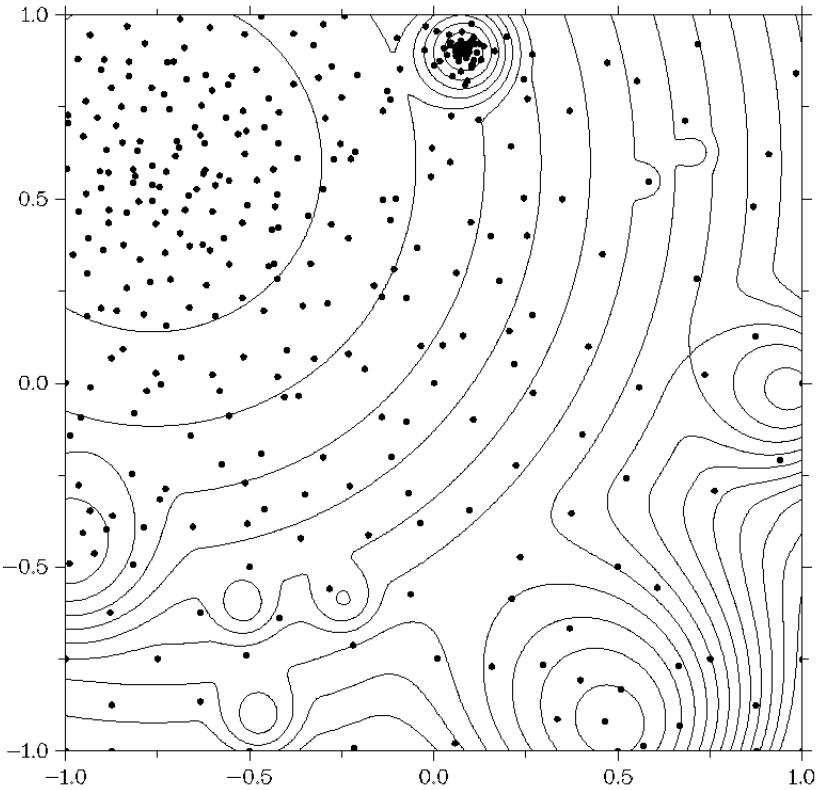
\includegraphics[width=0.45\textwidth]{isolines.png}
		\caption{Решение двумерной задачи}\label{fig:isolines}
\end{figure}
\par
Для примера на рис. \ref{fig:isolines} приведены линии уровня двумерной функции, порождаемой GKLS-генератором. Темные точки соответствуют 464 испытаниям, потребовавшимся для решения данной задачи с точностью 0.01 по координате; при этом число итераций составило 58 (на каждой итерации проводилось 8 испытаний). Линии уровня наглядно демонстрируют многоэкстремальность задачи, а расположение точек --- неравномерное покрытие, сгущающееся только в районе глобального минимума.
\par
Ниже приведены результаты численного сравнения трех последовательных алгоритмов --- DIRECT \cite{zilinsk}, DIRECT\(l\)  \cite{sergKvaDiaPaper} и алгоритма глобального поиска (АГП) (результаты работы первых двух алгоритмов приводятся по работе \cite{jonesLipOpt}). Численное сравнение проводилось на классах функций Simple и Hard размерности 4 и 5 из \cite{jonesLipOpt}. Глобальный минимум \(y^*\) считался найденным, если алгоритм генерировал точку испытания \(y_k\) в \(\delta\)-окрестности глобального минимума, т.е. \(\Vert y_k-y^*\Vert\leqslant\delta\). При этом размер окрестности выбирался (в соответствии с \cite{jonesLipOpt}) как \(\delta=\Vert b-a\Vert \sqrt[N]{\Delta}\), здесь \(N\) --- размерность решаемой задачи, \(a\) и \(b\) --- границы области поиска \(D\), параметр \(\Delta=10^{-6}\) при \(N=4\) и \(\Delta=10^{-7}\) при \(N=5\). При использовании метода АГП для класса Simple выбирался параметр \(r=4.5\), для класса Hard --- \(r=5.6\); параметр построения кривой Пеано был фиксированный \(m=10\). Максимально допустимое число итераций составляло \(K_{max} = 1 000 000\).
\par
В таблице 1 отражено среднее число итераций \(k_{av}\), которые выполнил метод при решении серии задач из данных классов. Символ «>» отражает ситуацию, когда не все задачи класса были решены каким-либо методом. Это означает, что алгоритм был остановлен по причине достижения максимально допустимого числа итераций \(K_{max}\). В этом случае значение \(K_{max}=1 000 000\) использовалось при вычислении среднего значения числа итераций \(k_{av}\), что соответствует нижней оценке этого среднего значения. Количество нерешенных задач указано в скобках.
\begin{table}
    \centering
    \begin{tabular}{|c|p{3cm}|c|c|c|}
    \hline
    \(N\) & Класс функций & DIRECT & DIRECT\(l\) & АГП \\ \hline
    4 & Simple & >47282 (4) & 18983 & 11953\\ \cline{2-5}
      & Hard & >95708 (7) & 68754 & 68754\\ \hline
    5 & Simple & >16057 (1) & 16758 & 15920\\ \cline{2-5}
      & Hard & >217215 (16) & >269064 (4) & >148342 (4)\\ \hline
    \end{tabular}
    \caption{Среднее число итераций}
    \label{table:average_iters}
\end{table}
\par
Как видно из таблицы \ref{table:average_iters}, АГП превосходит методы DIRECT и DIRECT\(l\) на всех классах задач по среднему числу итераций. При этом в классе 5-Hard каждый из методов решил не все задачи: DIRECT не решил 16 задач, DIRECT\(l\) и АГП – по 4 задачи.
\subsection{Задачи с трудоемким критерием}
Вначале приведем результаты экспериментов, которые соответствуют задачам с большим временем проведения одного поискового испытания. Оценим ускорение параллельного алгоритм глобального поиска (ПАГП), реализованного на CPU, в зависимости от использованного количества ядер \(p\). В таблицах \ref{table:time_speedUp_cpu} и \ref{table:iterations_speedUp_cpu} приведено ускорение по времени \(S(p)\) и по итерациям \(s(p)\). Ускорение вычислено относительно однопоточного запуска.
\begin{table}
    \centering
    \begin{tabular}{|c|c|c|c|c|}
    \hline
    \(p\) & \multicolumn{2}{|c|}{\(N=4\)} & \multicolumn{2}{|c|}{\(N=5\)}\\ \cline{2-5}
    & Simple & Hard & Simple & Hard \\ \hline
    2 & 2.45 & 2.20 & 1.15 & 1.32\\ \hline
	4 & 4.66 & 3.90 & 2.82 & 2.59\\ \hline
	8 & 7.13 & 7.35 & 3.47 & 5.34\\ \hline
    \end{tabular}
    \caption{Ускорение по времени \(S(p)\) на CPU}
    \label{table:time_speedUp_cpu}
\end{table}
\begin{table}
    \centering
    \begin{tabular}{|c|c|c|c|c|}
    \hline
    \(p\) & \multicolumn{2}{|c|}{\(N=4\)} & \multicolumn{2}{|c|}{\(N=5\)}\\ \cline{2-5}
    & Simple & Hard & Simple & Hard \\ \hline
	2 & 2.51 & 2.26 & 1.19 & 1.36\\ \hline
	4 & 5.04 & 4.23 & 3.06 & 2.86\\ \hline
	8 & 8.58 & 8.79 & 4.22 & 6.56\\ \hline
    \end{tabular}
    \caption{Ускорение по итерациям \(s(p)\) на CPU}
    \label{table:iterations_speedUp_cpu}
\end{table}
\par
Результаты экспериментов показывают значительное ускорение ПАГП при использовании CPU. Лучшие результаты получены при использовании всех ядер процессора.
\par
Далее изложим результаты экспериментов, проведенных с использованием Intel Xeon Phi. Вначале рассмотрим эксперименты на одном Xeon Phi в режиме Offload. Варьировалось количество потоков на сопроцессоре, все остальные параметры совпадают с предыдущими запусками. Приведено (таблицы \ref{table:time_speedUp_phi} и \ref{table:iterations_speedUp_phi}) ускорение относительно восьмипоточного запуска на центральном процессоре.
\begin{table}
    \centering
    \begin{tabular}{|c|c|c|c|c|}
    \hline
    \(p\) & \multicolumn{2}{|c|}{\(N=4\)} & \multicolumn{2}{|c|}{\(N=5\)}\\ \cline{2-5}
    & Simple & Hard & Simple & Hard \\ \hline
	60 & 0.54 & 1.02 & 1.07 & 1.61\\ \hline
	120 & 0.55 & 1.17 & 1.05 & 2.61\\ \hline
	240 & 0.51 & 1.06 & 1.07 & 4.17\\ \hline
    \end{tabular}
    \caption{Ускорение по времени \(S(p)\) на Phi}
    \label{table:time_speedUp_phi}
\end{table}
\begin{table}
    \centering
    \begin{tabular}{|c|c|c|c|c|}
    \hline
    \(p\) & \multicolumn{2}{|c|}{\(N=4\)} & \multicolumn{2}{|c|}{\(N=5\)}\\ \cline{2-5}
    & Simple & Hard & Simple & Hard \\ \hline
	60 & 8.13 & 7.32 & 9.87 & 6.55 \\ \hline
	120 & 16.33 & 15.82 & 15.15 & 17.31 \\ \hline
	240 & 33.07 & 27.79 & 38.80 & 59.31 \\ \hline
    \end{tabular}
    \caption{Ускорение по итерациям \(s(p)\) на Phi}
    \label{table:iterations_speedUp_phi}
\end{table}
\par
Результаты экспериментов показывают, что только на классе Simple при \(N=4\) реализация на Xeon Phi медленнее, чем CPU реализация, на классе Hard при \(N=4\) и на классе Simple при \(N=5\) версии для Xeon Phi и CPU демонстрирует примерно равную эффективность, а на классе Hard при \(N=5\) версия для Xeon Phi существенно превосходит CPU-реализацию. Наибольшее преимущество реализация для Xeon Phi показывает при 120 потоках для четырехмерных задач и при 240 потоках для пятимерных. При этом на всех классах наблюдается значительное ускорение по итерациям, а также практически линейная масштабируемость от числа потоков.
\par
Далее рассмотрим эксперименты с запуском сопроцессора в режиме MPI. Число уровней вложенности разбиваемой задачи равно двум. Число процессов, запущенных на сопроцессоре, –-- 30 (таблицы \ref{table:time_speedUp_phi_30mpi} и \ref{table:iterations_speedUp_phi_30mpi}) и 60(таблицы \ref{table:time_speedUp_phi_60mpi} и \ref{table:iterations_speedUp_phi_60mpi}), что соответствует ситуации, когда у корня дерева имеется соответственно 30 и 60 потомков. Процессы, работающие на сопроцессоре, использовали OpenMP для параллельного вычисления значений функции. Ускорение приведено относительно восьмипоточного запуска на CPU.
\begin{table}
    \centering
    \begin{tabular}{|c|c|c|c|c|}
    \hline
    \(p\) & \multicolumn{2}{|c|}{\(N=4\)} & \multicolumn{2}{|c|}{\(N=5\)}\\ \cline{2-5}
    & Simple & Hard & Simple & Hard \\ \hline
	4 & 3,18 & 5,14 & 5,15 & 14,65 \\ \hline
	8 & 3,53 & 1,49 & 3,35 & 10,49 \\ \hline
	16 & 1,09 & 2,77 & 4,61 & 14,36 \\ \hline
    \end{tabular}
    \caption{Ускорение по времени \(S(p)\) на Phi, 30 MPI процессов}
    \label{table:time_speedUp_phi_30mpi}
\end{table}
\begin{table}
    \centering
    \begin{tabular}{|c|c|c|c|c|}
    \hline
    \(p\) & \multicolumn{2}{|c|}{\(N=4\)} & \multicolumn{2}{|c|}{\(N=5\)}\\ \cline{2-5}
	4 & 11,19 & 19,19 & 9,27 & 27,38 \\ \hline
	8 & 13,97 & 3,63 & 8,24 & 23,85 \\ \hline
	16 & 1,29 & 3,56 & 8,28 & 22,12 \\ \hline
	\end{tabular}
    \caption{Ускорение по итерациям \(s(p)\) на Phi, 30 MPI процессов}
    \label{table:iterations_speedUp_phi_30mpi}
\end{table}
\begin{table}
    \centering
    \begin{tabular}{|c|c|c|c|c|}
    \hline
    \(p\) & \multicolumn{2}{|c|}{\(N=4\)} & \multicolumn{2}{|c|}{\(N=5\)}\\ \cline{2-5}
    & Simple & Hard & Simple & Hard \\ \hline
	4 & 2,76 & 3,20 & 4,19 & 16,56 \\ \hline
	8 & 3,05 & 7,73 & 4,08 & 14,87 \\ \hline
	16 & 0,89 & 5,21 & 2,72 & 13,05 \\ \hline
    \end{tabular}
    \caption{Ускорение по времени \(S(p)\) на Phi, 60 MPI процессов}
    \label{table:time_speedUp_phi_60mpi}
\end{table}
\begin{table}
    \centering
    \begin{tabular}{|c|c|c|c|c|}
    \hline
    \(p\) & \multicolumn{2}{|c|}{\(N=4\)} & \multicolumn{2}{|c|}{\(N=5\)}\\ \cline{2-5}
	4 & 10,36 & 3,34 & 6,01 & 26,04 \\ \hline
	8 & 9,04 & 28,81 & 7,68 & 25,02 \\ \hline
	16 & 1,27 & 28,66 & 7,19 & 30,38 \\ \hline
	\end{tabular}
    \caption{Ускорение по итерациям \(s(p)\) на Phi, 60 MPI процессов}
    \label{table:iterations_speedUp_phi_60mpi}
\end{table}
\par
Результаты экспериментов показывают, что запуск в режиме MPI значительно превосходит Offload режим по времени работы, однако проигрывает по числу итераций. Лучшие результаты для простого класса задач наблюдаются при использовании 30 процессов на сопроцессоре, а для сложного класса, при 60 процессах. Таким образом, можно сделать вывод, что задачи с большим временем работы, для которых важно число итераций метода оптимизации, лучше использовать запуск в режиме Offload, а для более быстро решаемых задач, лучше подходит режим MPI. 
\subsection{Задачи с легко вычисляемым критерием}
Рассмотрим теперь решение задач, в которых поисковые испытания проводятся быстро. Вначале приведем результаты OpenMP версии. В таблице \ref{table:time_speedUp_cpu_2} приведено ускорение относительно однопоточного запуска.
\begin{table}
    \centering
    \begin{tabular}{|c|c|c|c|c|}
    \hline
    \(p\) & \multicolumn{2}{|c|}{\(N=4\)} & \multicolumn{2}{|c|}{\(N=5\)}\\ \cline{2-5}
    & Simple & Hard & Simple & Hard \\ \hline
	2 & 1,09 & 1,09 & 0,56 & 0,57 \\ \hline
	4 & 1,10 & 1,06 & 0,74 & 0,66 \\ \hline
	8 & 0,90 & 1,11 & 0,45 & 1,77 \\ \hline
	16 & 0,66 & 0,92 & 0,76 & 0,66 \\ \hline
	32 & 0,29 & 0,38 & 0,22 & 0,55 \\ \hline
    \end{tabular}
    \caption{Ускорение по времени \(S(p)\) на CPU}
    \label{table:time_speedUp_cpu_2}
\end{table}
\par
Эксперименты показывают незначительное ускорение, а во многих случаях – и замедление при вычислениях только на центральном процессоре.
\par
Далее рассмотрим ускорение при использовании Xeon Phi в режиме MPI. Результаты приведены относительно однопоточного запуска на CPU. В таблице \ref{table:time_speedUp_phi_30mpi_easy} приведено ускорение по времени \(S(p)\) для запуска 30 процессов на Xeon Phi, в таблице \ref{table:time_speedUp_phi_60mpi_easy} для 60 процессов.
\begin{table}
    \centering
    \begin{tabular}{|c|c|c|c|c|}
    \hline
    \(p\) & \multicolumn{2}{|c|}{\(N=4\)} & \multicolumn{2}{|c|}{\(N=5\)}\\ \cline{2-5}
    & Simple & Hard & Simple & Hard \\ \hline
	1 & 0,35 & 2,28 & 0,37 & 1,92 \\ \hline
	2 & 0,94 & 1,95 & 0,39 & 1,23 \\ \hline
	4 & 1,23 & 0,43 & 0,54 & 2,63 \\ \hline
	8 & 0,85 & 0,56 & 0,40 & 1,53 \\ \hline
	\end{tabular}
    \caption{Ускорение по времени \(S(p)\) на Phi, 30 MPI процессов}
    \label{table:time_speedUp_phi_30mpi_easy}
\end{table}
\begin{table}
    \centering
    \begin{tabular}{|c|c|c|c|c|}
    \hline
    \(p\) & \multicolumn{2}{|c|}{\(N=4\)} & \multicolumn{2}{|c|}{\(N=5\)}\\ \cline{2-5}
    & Simple & Hard & Simple & Hard \\ \hline
	1 & 0,59 & 2,56 & 1,22 & 3,30 \\ \hline
	2 & 0,89 & 0,87 & 1,29 & 2,76 \\ \hline
	4 & 1,09 & 1,03 & 0,38 & 5,32 \\ \hline
	8 & 0,70 & 0,78 & 0,69 & 2,19 \\ \hline
	\end{tabular}
    \caption{Ускорение по времени \(S(p)\) на Phi, 60 MPI процессов}
    \label{table:time_speedUp_phi_60mpi_easy}
\end{table}
\par
Результаты экспериментов показывают ускорение на Xeon Phi, превосходящее ускорение на центральном процессоре. Лучшие результаты получены при использовании 30 процессов на Xeon Phi только для простых четырехмерных задач, все остальные задачи лучше всего решаются при использовании 60 процессов.
\par
Теперь перейдем к эксперименту с шестимерными задачами простого класса. При решении шестимерной задачи с использованием одного процесса (вложенные подзадачи отсутствуют) и сохранением точности построения развертки \(m=10\) требуется использовать числа с плавающей запятой расширенной точности, что ведет к значительному увеличению времени работы алгоритма. При этом в случае использования хотя бы одного уровня вложенных подзадач, задачи на каждом уровне будут решаться без подключения расширенной точности, что обеспечивает дополнительное преимущество блочной многошаговой схемы.
\par
Рассмотрим результаты эксперимента с использованием Xeon Phi в режиме MPI, таблица \ref{table:time_speedUp_phi_2}. Число уровней вложенности разбиваемой задачи равно двум. Приведены результаты экспериментов для разбиений 3:3 (три переменных на первом уровне, три – на втором) и 4:2 (4 переменных на первом уровне, две – на втором). Число процессов, запущенных на сопроцессоре равно 30 и 60, что соответствует тому, что у корня дерева имеется соответственно 30 и 60 потомков. Процессы, работающие на Xeon Phi, использовали OpenMP для параллельного вычисления значений функции. Ускорение приведено относительно однопоточного запуска на CPU.
\begin{table}
    \centering
    \begin{tabular}{|c|c|c|c|c|}
    \hline
    \(p\) & \multicolumn{2}{|c|}{30 процессов} & \multicolumn{2}{|c|}{60 процессов}\\ \cline{2-5}
	& 3:3 & 4:2 & 3:3 & 4:2 \\ \hline
	2 & 7,30 & 9,87 & 17,68 & 18,21 \\ \hline
	4 & 5,99 & 8,18 & 6,60 & 13,57 \\ \hline
	8 & 3,14 & 12,74 & 5,92 & 25,58 \\ \hline
	16 & 3,54 & 7,61 & 4,87 & 11,33 \\ \hline
	32 & 3,41 & 6,85 & 3,73 & 6,50 \\ \hline
\end{tabular}
    \caption{Ускорение по времени \(S(p)\) на Phi}
    \label{table:time_speedUp_phi_2}
\end{table}
\par
Результаты экспериментов показывают значительное ускорение запуска на сопроцессоре по сравнению с запуском только на центральном процессоре. Лучшее ускорение наблюдается при шестидесяти MPI процессах на Xeon Phi по 8 потоков на каждый процесс, время работы в 25 раз меньше, чем решение задачи только на центральном процессоре.

\section{Заключение}
В работе рассмотрен параллельный алгоритм глобального поиска, разработанный в рамках информационно статистического подхода. Предложен подход к распараллеливанию данного алгоритма, который может быть эффективен как в задачах с трудоемким критерием оптимизации, так и в задачах с относительно простым критерием. Проведены эксперименты с реализацией предложенного параллельного алгоритма на суперкомпьютере «Лобачевский» с использованием сопроцессоров Intel Xeon Phi. Результаты вычислительных экспериментов подтверждают высокую эффективность распараллеливания для Xeon Phi во всех классах рассмотренных задач.

\bibliography{refs}

\end{document}